\chapter{User Study}

We conduct an user study above alternative design from April 14, 2016 to April 15, 2016, which is located at the Southwest University for Nationalities Wuhou Campus Bibliothek ground floor reading room.
%我们在 2016 年 4 月 14 日至 2016 年 4 月 15 日将上述备择设计实施了一个长达两天 (19:00 至 22:00) 的用户调研,其地点位于西南民族大学武侯校区图书馆一层阅览室。

\section{User Tasks}

In this study, there are five operation we need to evaluate: tap, force touch, digital crown, swipe left and swipe right. According this, we designed two completely group tasks, and they are Calling(two way to archive) switch watch digital plate. These tasks are above five operations combinations.
%在调研中,一共需要评估备择设计中的五种操作设计:轻触、重触、调节旋钮、左滑、右滑。据此,我们设计了两种不同的完整任务,分别是拨打电话(两种方式)和更换表盘界面。总共三个基本任务的执行涵盖了上述五种操作。%,对于拨打电话任务而言,用户有两种方式实施任务。

\begin{itemize}
    \kaishu
    \item \textbf{Task 1}: Use side button. Find top contacts, then select a person and make the call. The task logic is rise hand first, push the side button and then rotate Digital Crown to select a person, tap to select this person and make the phone call.
    %任务一:拨打电话的第一种方式是使用侧面按钮,找到常用联系人,然后拨号。其中的任务逻辑为:抬起手腕,呼出常用联系人(点击侧面按钮),旋转旋钮选择联系人(旋转旋钮),点击联系人头像(点击屏幕),点击拨打电话(点击屏幕),选择号码(点击屏幕),完成;
    \item \textbf{Task 2}: Use Call App. Push Digital Crown enter into Application desktop first, tap Call App then make the phone call. The task logic is rise hand first, click Digital Crown, tap screen to select Call App, select a person and then tap to make a phone call.
    %任务二:而第二种方法则是从表盘界面进入总应用界面,从总应用界面选择电话应用进行拨号。其中的任务逻辑为:抬起手腕,进入 App 总界面(点击旋钮),选择电话(点击屏幕),点击最近联系人(点击屏幕),点击联系人(点击屏幕),完成;
    \item \textbf{Task 3}: The task of switch watch layout is simple than the other two tasks. The most important operation is make a Force Touch on watch screen. The task logic is rise hand first, make a Force Touch on watch screen, and swipe to left or right change its interface, then tap the screen and finish this task.
    %任务三:更换表盘的任务则比较简单,只需要在表盘界面使用 Force Touch 即能进行更换。其中的任务逻辑为:抬起手腕,用力按压屏幕(Force Touch),手指向左滑动(左滑),点击屏幕(点按),完成。
\end{itemize}

Before starting user tasks, we teach our participants about how to interact on a smart watch, and teach them 13 gestures without any hint of alternative design, gestures are list on Table \ref{table:gesture}. We start the user study until we make sure they can interact with Apple Watch well and also remembered these 13 gestures.
%在开始任务之前,用户会学习手表的基本操作,并在用户不知情的情况下学习拇指与其他手指快速捏合、拇指与其他手指用力捏合、拇指在其他手指上的滑动以及五根手指从伸展到握拳攻击十三种手势,如表\ref{table:gesture}所示。在确认操作无障碍后,才确认开始实验。

\begin{table}[H]
    %\scriptsize
    \small
    \kaishu
    \centering
    \setlength{\belowcaptionskip}{10pt}
    \caption{Gestures Index}

    \begin{tabular}{c l}
        \toprule
        \textbf{Index}        & \textbf{Description} \\
        \hline
        1     & Thumb swipe on index finger \\
        2     & Thumb swipe on middle finger \\
        3     & Thumb swipe on ring finger \\
        4     & Thumb swipe on little finger \\
        5     & Thumb pinch with index finger \\
        6     & Thumb force pinch with index finger \\
        7     & Thumb pinch with middle finger \\
        8     & Thumb force pinch with middle finger  \\
        9     & Thumb pinch with ring finger  \\
        10    & Thumb force pinch with ring finger \\
        11    & Thumb pinch with little finger \\
        12    & Thumb force pinch with little finger \\
        13    & Five fingers grab \\
        \bottomrule
    \end{tabular}

    \label{table:gesture}
\end{table}

After above three tasks, we show the first part of questionnaire to participants, an requires participants recall previous learning of gesture and related tasks to complete this part of questionnaire. Then we goes to next stage of user tasks for alternative interaction:
%完成上述三个任务后,首先向用户出示调研问卷的第一部分,见附录\ref{appendix:b},并要求用户在回忆此前学习的手势和相关任务完成此部分问卷。完成这部分问卷后,再要求用户完成上述三个任务在备择设计下对应的任务。

\begin{itemize}
    \kaishu
    \item Alternative Task 1: raise hand, call Friends view (grab), choose contact (pinch), make phone call (pinch 3 times);
    %任务一的备择交互方式的操作逻辑是:抬起手腕,呼出常用联系人(握拳一次),选择联系人(拇指在食指上滑动),拨打电话(需要三次点击屏幕,即拇指和食指快速捏合三次);
    \item Alternative Task 2: raise hand, back to App homepage(grab 2 times), select phone App and make the phone call (pinch 3 times);
    %任务二的备择交互方式的操作逻辑是:抬起手腕,返回应用界面(握拳两次),完成电话拨打(需要三次点击屏幕,拇指和食指快速捏合三次);
    \item Alternative Task 3: raise hand, Force Touch (force pinch, long time), swipe to left or right (thumb and middle finger pinch), tap to end selection (pinch).
    %任务三的备择交互方式的操作逻辑是:抬起手腕,在表盘界面下进行 Force Touch (拇指和食指长时间捏合), 向左滑动(拇指和中指快速捏合),最后再轻点屏幕选择新的表盘(拇指和食指快速捏合)。
\end{itemize}

Alter these altetnative interaction task, we show the first part of survey again, requires participants mofify their answer until the answer satisfy their own. When this finished, we show the second part of quesionnaire, see Appendix \ref{appendix:c}, then we logout this user study.
%在完成备择交互方式的任务之后,再向用户出示问卷的第一部分,要求用户对此前的结果进行修改直至用户自身满意为止。完成后,向用户出示问卷的第二部分,见附录\ref{appendix:c},并在填写完成后结束本次实验。

\section{Participants}

Sample size of participants in a usability test sometimes do not have a fixed program, the classic theory is that usability test for serious usability problems can only take five participants\cite{albert2013measuring}. However, \cite{faulkerner} analysed increase sample size to 20 can find more than 95\% usability problems.
%可用性测试中参与者样本数的设置通常没有固定的方案,经典的可用性测试理论认为对于严重的可用性问题只需五名参与者即可被发现\cite{albert2013measuring}。但是,文\cite{faulkerner}详细分析了在可用性测试中增加用户样本数的具体好处,当参与者数量为20时,可以发现95\%的可用性测试问题。

Hwang et al.\cite{Hwang:2010:NPR:1735223.1735255} disscussed the changing rule of sample size in usability test. R. Macefield et al.\cite{Macefield:2009:SPG:2835425.2835429} gives the influence of sample size in each study group, they point out that 5 to 10 is the best base number in each study group.
\cite{medlock2002using} suggested use smaple ratio to evaluate sample size when the number of evaluate task is inequal to user tasks per user.
%Hwang 等人在\cite{Hwang:2010:NPR:1735223.1735255}中讨论了并给出了可用性测试中在样本数设置的变动规则。
%R. Macefield 等在 \cite{Macefield:2009:SPG:2835425.2835429}讨论了每个用户组中参与者个数的设置对参与者样本数量的影响,并指出将每一组的用户基数设置为5至10人是较为合理的方式。
%\cite{medlock2002using} 讨论了评估的总任务和用户任务数量存在差异时,通过引入比例来调整用户样本大小。

In \cite{pernice2009eyetracking}, they disscussed how eye tracking influence the usability test. The above discussion of its literature, we conclude that given an algorithm \ref{alg:participant} as usability testing sample size calculation method. Wherein calculating the number of samples is determined by the following parameters:
%最后,在文\cite{pernice2009eyetracking}中则讨论了当可用性测试中引入眼球追踪时对参与者样本的影响。综合上述文献的讨论,我们总结给出算法\ref{alg:participant}作为可用性测试中参与样本大小计算方法。其中,样本数的计算由以下几个参数决定:
\begin{enumerate}
    \kaishu
    \item \textbf{group}: number of user group(such as expert or freshman), this number should not large than 5;
    %用户组的数量(专家、新手等),用户组数量不因超过五组;
    \item \textbf{task}: Is the user task same between different group?
    %不同组之间的用户任务是否相同;
    \item \textbf{baseline}: Will user study result influence product decision or not?
    %实验结果是否会影响未来产品决策;
    \item \textbf{design}: evaluating design numbers in a user study, this number should not large than 5;
    %一次调研中需要比较多少种不同的设计,比较的设计不应超过五种;
    \item \textbf{peruser}: evaluating design number for each user, each user should not evaluate more than 5 design;
    %每个用户需要评估多少种设计,用户需要评估的设计不应超过五种;
    \item \textbf{eyetracking}: Is this user study enable eye tracking? If so, is it qualitatively or quantitatively?
    %是否在实验中使用眼球追踪,当支持时,因确定其追踪目的为定性(qualitatively)还是定量(quantitatively)。
\end{enumerate}

Then we have the algorithm of participants sample size in usability test:
%而可用性测试中参与者数量的算法为:

\begin{algorithm}[H]
\caption{Calculate minimum participant sample size}
\label{alg:participant}
\begin{algorithmic}
\REQUIRE $group, task, design, peruser, eyetracking$
\ENSURE $sample$
\STATE $base \leftarrow 10$
\STATE $sample \leftarrow 10$
\IF{eyetracking is qualitatively}
\STATE $base \leftarrow 12$
\ELSIF{eyetracking is quantitatively}
\STATE $base \leftarrow 39$
\ENDIF
\IF{baseline is yes}
\STATE $base \leftarrow 16$
\ENDIF
\IF{$design \leq peruser$}
\STATE $ratio \leftarrow 1$
\ELSE
\STATE $ratio \leftarrow \lfloor\frac{\text{design}}{\text{peruser}}\rfloor$
\ENDIF
\IF{task is same}
    \STATE $sample = \lceil (base + 6 \cdot (group - 1)) \cdot ratio \rceil$
\ELSE
    \STATE $sample = \lceil base \cdot group \cdot ratio \rceil$
\ENDIF
\end{algorithmic}
\end{algorithm}

In our user study, we randomly invite participants perform same tasks, and the results influences future design, so the perameters are $\text{group}=1, \text{baseline}=\text{yes}, \text{task}=\text{same}, \text{design}=5, \text{peruser}=5, \text{eyetracking}=\text{no}$. According to algorithm \ref{alg:participant}, the sample size should not smaller than 16. We put this user study information in social networks and also randomly invite people who get in or out from library become a participant, and finally we have 21 participants.
%在本次用户调研中,我们随机地邀请参与者执行相同的任务,且实验结果会影响未来的设计形式。因此 $\text{group}=1, \text{baseline}=\text{yes}, \text{task}=\text{same}, \text{design}=5, \text{peruser}=5, \text{eyetracking}=\text{no}$ 。根据算法\ref{alg:participant}容易算出,合适的样本数应不小于 16 。我们在社交网络上发布参与调研的相关信息,并对进入图书馆或离开图书馆的行人进行随机邀请,一共取得了 21 位参与者。

\section{Analysis and Results}

\subsection{Statistics of Participants}

Out of 21 participants, 11 were male and 10 were female. The range of age was 18 to 28. Besides, there are three participants have smart watch use experiences.
%在 21 名参与者中,其年龄范围在 18 至 28 之间。%,分布情况如图\ref{fig:age-dist}所示,
%其中男性 11 人,女性 10 人。此外,在这些参与者中,共有三名参与者有智能手表的使用经验。

Participants who have use watch in daily life all own more than two watches, and there are 9 participants consider to buy a smart watch. In watch users, only 6 participants plan to buy a smart watch and most of them regard its prices.
%在这部分参与者中,有 12 名参与者在日常生活中使用手表,并平均拥有过两款以上的手表。
%有 9 位参与者打算在未来考虑购买智能手表,而在已经在使用手表的参与者中,有 6 位在未来考虑购买智能手表,并且这部分人认为最影响其使用智能手表的因素为价格。

We have 26.57\% (6 people) participants neither do not have a watch or do not consider to buy it. In another words, they will never buy a smart watch if smart watches is not a necessary product.
%在没有手表也没有购买智能手表意愿的28.57\%的参与者中(共6人),均为没有手表使用习惯的用户,换句话说,如果智能手表不能成为生活必需品,那么几乎不太可能获得这部分用户。

% \begin{figure}[H]
%     \kaishu
%     \centering
%     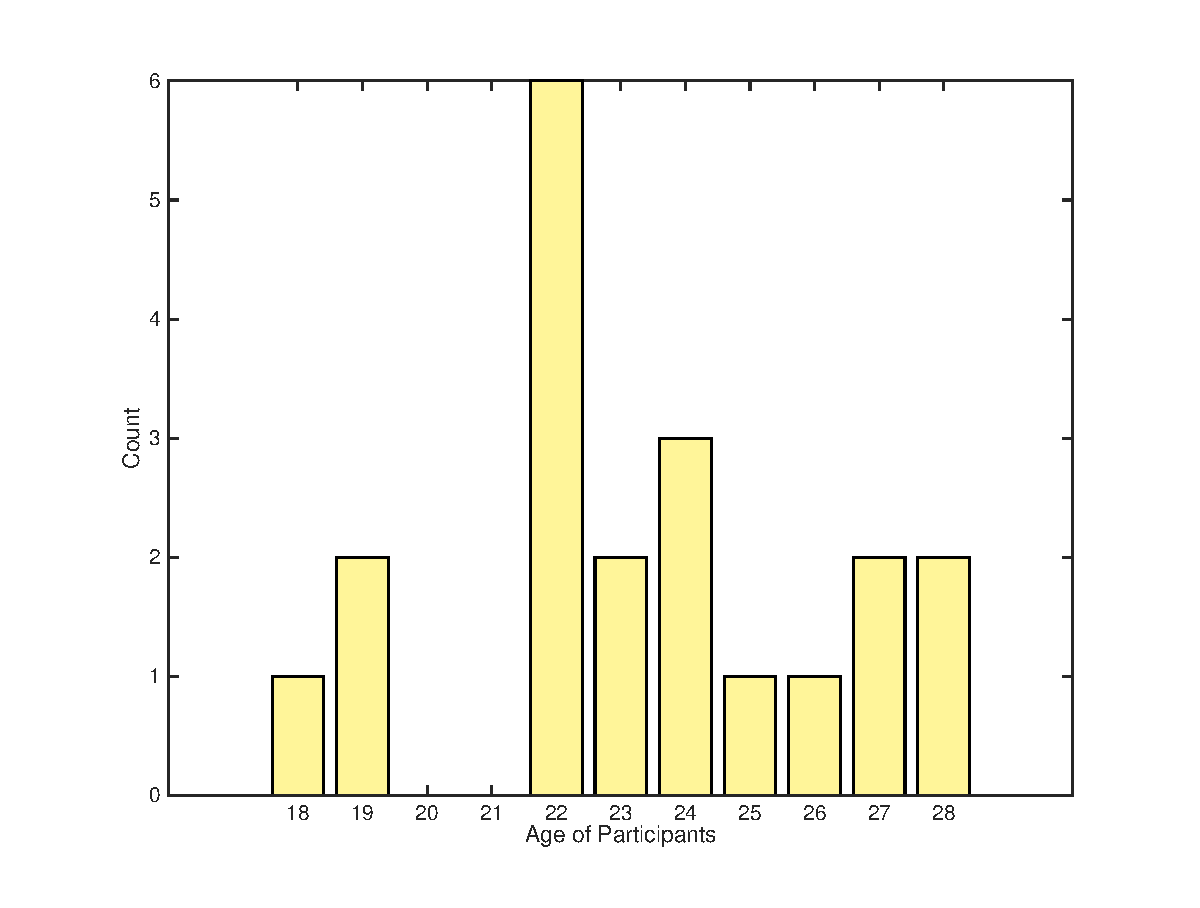
\includegraphics[width=0.5\textwidth]{figures/age-dist}
%     \caption{\kaishu 参与者年龄分布}
%     \label{fig:age-dist}
% \end{figure}

\subsection{Social Acceptable}

In the first part of questionnaire, we set up a social acceptability problem, it is "how to treat strangers raise hand excuse gestures in Table \ref{table:gesture}?". In these participants, there are 42.85\% (8 people) participants thought it was exercise, 14.28\% (3 people) thought it was thinking, and 33.33\% (7 people) thought it was a performance art, 19.04\% (4 people) didn't care about it and 4.76\% (1 person) considered "insane".
%在问卷的第一部分中,我们设置了对社会接受性考察的问题,问题设置为『如何看待公共场合陌生人抬起手腕执行表\ref{table:gesture}所示手势』。在二十一位参与者中,有42.85\%的参与者(8人)认为是在锻炼或活动手部,有14.28\%的参与者(3人)认为在进行思考,有33.33\%的参与者(7人)认为这种行为是一种行为艺术并对其表示好奇,而19.04\%的参与者(4人)对这种行为没有想法并不会在意,另外则有4.76\%的参与者(1人)认为可能是精神失常。

From the above results, all participants accept this action except 4.76\% (1 person).
%从上述结果来看,除了4.76\%的参与者对这种方式稍微不能接受外,其他参与者均对此种单手手势行为表示开放或接受态度。

\subsection{Comfortable Rate of Gestures}

% Participants in the first part of the questionnaire on the table \ ref {table: gesture} listed gestures of comfort voting results are shown in \ ref {fig: gesture-vote} shown.
Every participant makes a gestures comfort voting, gestures is in Table \ref{table:gesture}, results shown on Figure \ref{fig:gesture-vote}.
%参与者在问卷的第一部分中对表\ref{table:gesture}中所列手势进行了舒适程度投票,结果如图\ref{fig:gesture-vote}所示。

\begin{figure}[H]
    \kaishu
    \centering
    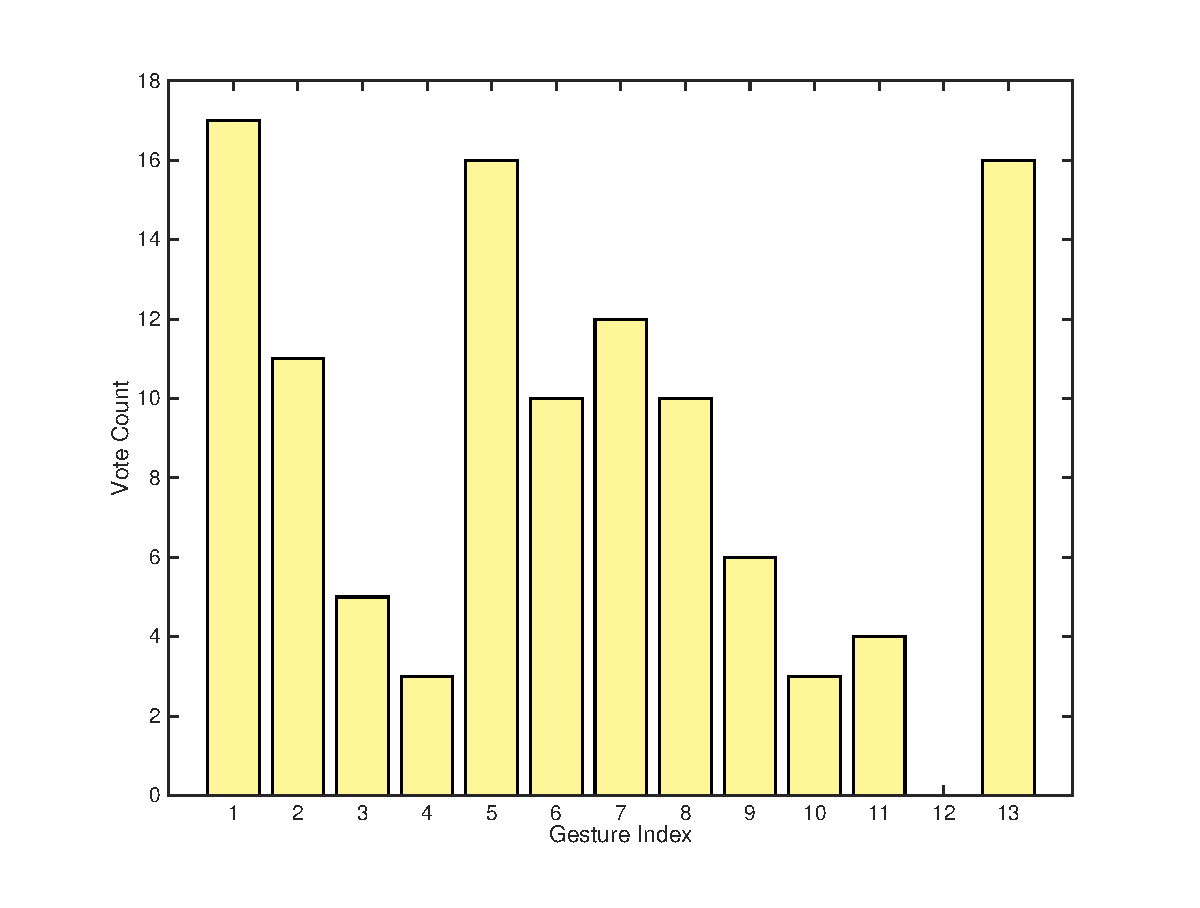
\includegraphics[width=0.5\textwidth]{figures/gesture-vote}
    \caption{\kaishu Vote results of gestures in Table \ref{table:gesture}}
    \label{fig:gesture-vote}
\end{figure}

The results showed that more than 16 people (76.19\%) vote three gestures, they are swipe between thumb and index finger, pinch with thumb and index finger and five finger grab, they are in the first echelon. Thus these three single hand gestures has comfortable and easy characteristics for users.
%结果显示,大拇指在食指上滑动、大拇指和食指的捏合、五根手指由伸展转变为握拳三个手势获得了最高且几乎一致的投票数(76.19\%, 大于16人),处于第一梯队。说明这三个单手手势在用户中普遍具有舒适和易接受的特性。

Next, the second echelon, more than 11 people (52.38\%) vote to thumb swipe on middle finger, long pinch with thumb and index finger. It is indicative that these gestures' comfort lower than the first echelon gesture.
%其次,拇指在中指上滑动、拇指和食指的长时间捏合、拇指和中指的快速及上时间捏合获得了第二梯度的票数(52.38\%, 大于11人),说明这部分手势舒适性次之,用户的使用频率不会高于第一梯队的手势。

It is worth to mention that in all 21 participants, no one choose thumb pinch with little finger, which means this gesture is the most uncomfortable gesture among them. In contrast, we can use this gesture to operate some dangerous operation, such as delete.
%值得一提的是,在全部 21 位参与者中,没有一人选择拇指和小指的捏合,即参与者普遍认为大拇指和小指的长时间捏合操作极不舒适,不适合用作常用的手势。相反,当进行一些比较危险的操作(如删除)时,可以考虑使用这个手势进行设计。

\subsection{Gesture Intuition}

We are also studied user's gesture intuition, to verify the reasonableness of the alternative design in the first part of questionnaire. Voting results as shown in Figure \ref{fig:heat}, in which the red color indicates more deeper gets gesture intuition for user more higher.
%我们还在问卷第一部分中考察了用户的手势操作直觉,用以验证备择设计的合理性。备择设计的五个基本操作轻点、Force Touch、Digital Crown 和屏幕滑动(左右滑动)中,参与者对十三个手势的投票结果如图\ref{fig:heat}所示,其中红色颜色越深表明用户直觉越高。

\begin{figure}[H]
    \kaishu
    \centering
    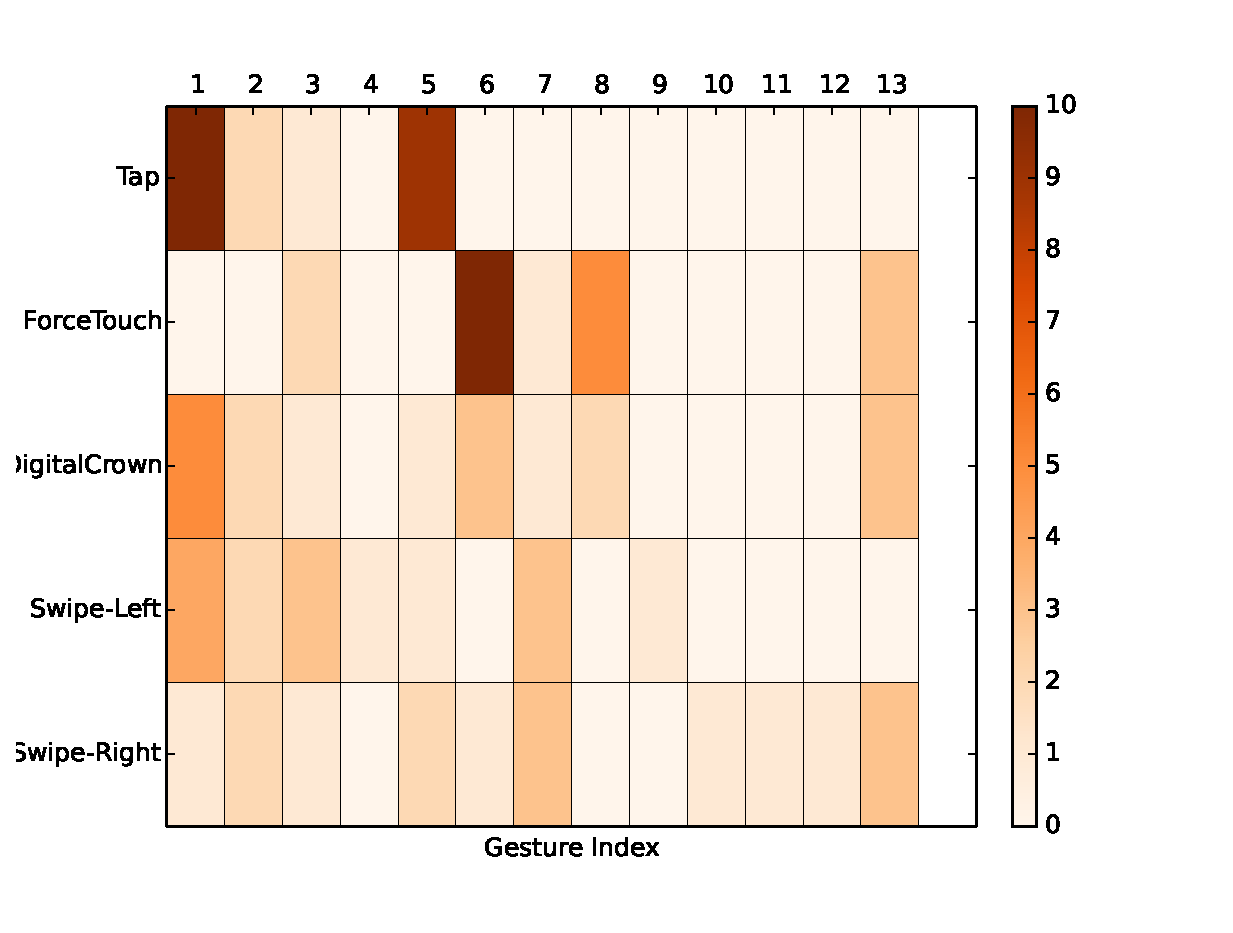
\includegraphics[width=0.5\textwidth]{figures/heat}
    \caption{\kaishu Heatmap of intuition vote results}
    \label{fig:heat}
\end{figure}

According to the results, participants thought the tap and force touch gestures is a strong intuitive operation. In tap gesture, participants has two obvious point of view, some may say thumb swipe on index finger is more intuition, and some may say quick pinch is more logical.
%从图中很容易看出,参与者对轻点、Force Touch 都有较为强的操作直觉。在轻点中,用户存在两个明显的分歧,有一部分人认为与轻点操作更加符合的操作逻辑应该是拇指和食指间的滑动,另一部分人则认为更合适的操作逻辑是拇指和食指的快速捏合。%出现这种情况的原因是:%*****(暂时没想明白为什么会这样。。)

Especially for Force Touch, the user does not exist distinct operation divisions. participants were generally more inclined to use long pinch. Digital Crown's gesture were more modest, but it can be observed that user tend to use thumb swipe on index finger.
%尤其是对 Force Touch ,用户之间不存在明显的操作分歧,参与者普遍较倾向于使用拇指和食指间的长时间点按进行操作。其对于 Digital Crown 的手势操作直觉则较适中,但能观察到用户倾向于使用拇指和食指的双指滑动。

However, for swipe gesture, participant becomes confused, there are no obvious results shows. So we still need to considering this part of gestures carefully, and sometimes we may need user to learn these gestures.
%然而,对于滑动操作来说,参与者的选择则开始变得迷惑,用户在多个不同的手势选择上飘忽不定,每种操作都有三种以上的不同手势被参与者选择。因此,对于滑动、返回这部分设计而言,可能需要用户进行一定程度上的学习才能获得较好的交互效果。

\section{Conclusions}

Performance by participants in this survey, we can conclude the alternative design of tap, Force Touch and Digital Crown is more comfortable and intuitive for user's operation. As it happens, this is the most frequency operation for smart watch interaction.
%通过本次调研中参与者的表现我们可以看到,在备择交互设计中,我们对于点按、Force Touch 和 Digital Crown 这部分交互方式是较为符合用户操作直觉、同时也是参与者认为较为舒适的手势操作。恰好,这部分操作正是用户与手表进行交互时最常用的操作。

For others, there is no obvious logic and intuition for interaction. Fortunately, the Apple Watch display content vertically so swipe left and right are not frequency, back to previous view belongs to a sensitive operation, we could use these gesture to improve user vigilance and pay more attention on it.
%而对于左右的滑动、返回、握拳实施特殊按钮这部分的设计,用户没有感受到较为明显的操作直觉和交互逻辑。幸运的是,在 Apple Watch 这种垂直方向上流式展示信息的设备上,左右滑动的交互不够常用,而返回操作属于较为敏感的操作,因此使用不太符合操作逻辑的操作反而能够提高用户警惕,防止误操作。

In consequences, our alternative interaction design is appropriate for most normal users.
%换句话说,作为备用的交互手段,其设计是良好的。

\cleardoublepage
